%# -*- coding: utf-8-unix -*-
% !TEX program = xelatex
% !TEX root = ../thesis.tex
% !TEX encoding = UTF-8 Unicode
%%==================================================
%% chapter02.tex for SJTU Master Thesis
%% based on CASthesis
%% modified by wei.jianwen@gmail.com
%% Encoding: UTF-8
%%==================================================

\chapter{基于深度强化学习的NL2SQL生成}
\label{chap:enl2sql}

\section{研究问题}

随着计算机技术的快速发展与应用,关系型数据库被广泛应用于教育、医疗、商业等领域。
作为信息存储的载体,越来越多的软件开发和业务人员正频繁使用SQL查询语句来读取关系型数据库中的数据。
SQL语句用法多样且功能强大,但对于一个没有技术背景的使用者来说却是一场噩梦。
即便是一名专业的软件人员,在面对数据库中众多的实体以及每个实体都有自己独特的含义时,想要把SQL语句写正确也不是一件容易的事情。
因此,学术界和工业界一直都在思考如何更快更好地使用SQL语句来读取数据,其中最理想和最直接的方式便是直接让使用者使用自然语言从数据库中获取所需信息。

实现这个目标的关键在于如何去理解自然语言语句的意图并讲其映射到SQL语句上,简称为NL2SQL(Nature Language To SQL Statement),即自然语言生成SQL查询语句任务。
在NL2SQL任务中,一个典型的例子如图\ref{fig:nl2sqlexample}给出。

\begin{figure}[!htp]
    \centering
    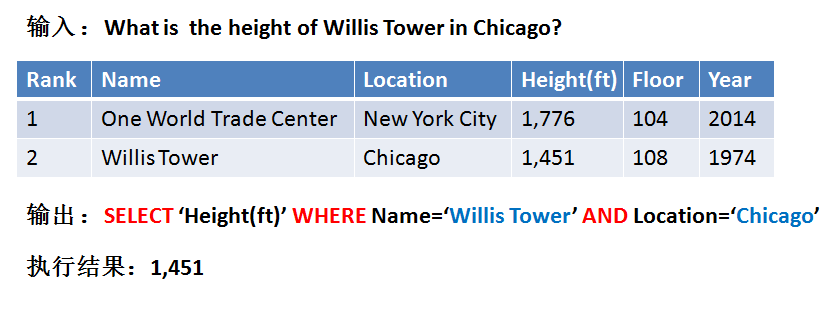
\includegraphics[width=15cm]{example/nl2sql.png}
    \bicaption[这里将出现在插图索引中]
      {NL2SQL的一个典型示例}
      {English caption}
    \label{fig:nl2sqlexample}
  \end{figure}

图\ref{fig:nl2sqlexample}为WikiSQL数据集[!!引用!!]中的一个样例。
WikiSQL数据集是纯自然语言生成SQL查询语句的第一个数据集。
其中包含80654组自然语言问句及其对应的SQL查询语句,涵盖24241张从Wikipedia中获取的数据表。
从图中可以看到,NL2SQL任务的输入实际包括两部分:自然语言问题以及一个简单的数据表schema(schema代表数据表及表中的列)。

WikiSQL数据集中SQL查询语句具有一定的约束条件,必须符合如下模板:

\begin{table}[!hpb]
    \centering
    \bicaption[指向一个表格的表目录索引]
      {SQL查询语句模板}
      {A Table}
    \label{nli:sqlmb}
    \begin{tabular}{@{}llr@{}} \toprule
      % \multicolumn{2}{c}{Item} \\ \cmidrule(r){1-2}
    %   节点类型 & 对应的SQL组件\\\midrule
    \emph{SELECT   agg   selcol   WHERE   col   op   val   (AND   col   op   val)*}\\\bottomrule
  
      % Animal & Description & Price (\$)\\ \midrule
      % Gnat & per gram & 13.65 \\
      % & each & 0.01 \\
      % Gnu & stuffed & 92.50 \\
      % Emu & stuffed & 33.33 \\
      % Armadillo & frozen & 8.99 \\ \bottomrule
    \end{tabular}
  \end{table}

  在\ref{nli:sqlmb}中,\emph{selcol}代表表中的列名,\emph{agg}代表聚合操作(例如:COUNT,SUM或空),
  \emph{WHERE}后面为由一系列过滤调教构成的子句,每个\emph{op}代表一个过滤操作(例如:“=”),\emph{val}代表出现在自然语言问句中的过滤值。
  值得注意的是,尽管模板中的过滤条件服从标准的线性顺序,但由于存在\emph{AND}符号,所以过滤条件的先后顺序是无关紧要的。

  在后文中,我们声明如下一些表示:总输入表示为$x$,其包含由单词$w_{i}$组成的自然语言问题$w$以及由列名$c_{j}$组成的单张表的schema $c$(其中,列名$c_{j}$可由单个或多个单词组成)。
  最后,我们的模型需要生成一条可执行的SQL查询语句$y$作为输出。

\section{相关技术}
\subsection{NL2SQL研究现状}
\subsection{深度学习}
\subsection{强化学习}
\subsection{语义解析}
\section{解决方案}

\subsection{增强解析器模型}
\label{enl2sql:zqjxqmx}
针对每个输入$x$来生成结构化的输出$y$的过程可以被分解成为一系列的语义解析决策的过程。
所以,增强解析器模型的基本思路为:解析器从初始状态启动并不断根据学习的策略采取不同的操作。
每个动作(action)都会将解析器从一个状态(state)转移为另一个状态,知道解析器到达它的最终状态并停止。
在解析器的最终状态下,我们可以获取一个完整的输出$y$。
我们采取一种概率的方法来对整个的策略(policy)建模。
它可以对由输入$x$产生的有效的动作(action)的集合以及解码器产生的历史行为进行概率分布进行预测。
所以,整个增量语义解析器的训练目标就转换为了如何优化一个参数化的策略的问题。

% , 其中$\theta$为模型参数。
\begin{equation}
    \label{enl2sql:eq1}
    % Sim \left ( n ,\right v) = \max\left ( Sim_{wup}\left ( n ,\right v) ,\right Sim_{gram}\left ( n ,\right v))
    % Sim(n,v) = \max(Sim_{wup}(n,v),Sim_{gram}(n,v))
    % P_{\theta}(y|x) = P_{\theta}(\boldsymbol{a}|x),   \theta为模型参数
    P_{\theta}(y|x) = P_{\theta}(\boldsymbol{a}|x),  \qquad \theta\text{为模型参数}
\end{equation}

根据公式\ref{enl2sql:eq1},通过执行动作(action)序列$\boldsymbol{a} = \{a_{1},a_{2},...,a_{k}\}$,解析器将被不断引导并从初始状态转换为包含输出$y$的最终状态。
在此,我们需要假设每个输出$y$有且仅有一个对应的动作序列$\boldsymbol{a}$(详见\ref{enl2sql:ndo}节内容)。
行动序列的概率$P_{\theta}(\boldsymbol{a}|x)$可展开为增量策略概率的乘积(公式\ref{enl2sql:eq2}):

\begin{equation}
    \label{enl2sql:eq2}
    % Sim \left ( n ,\right v) = \max\left ( Sim_{wup}\left ( n ,\right v) ,\right Sim_{gram}\left ( n ,\right v))
    % Sim(n,v) = \max(Sim_{wup}(n,v),Sim_{gram}(n,v))
    P_{\theta}(\boldsymbol{a}|x) = \prod^k_{i=1}P_{\theta}(a_{i}|x,a_{<i}),   \qquad |\boldsymbol{a}| = k
\end{equation}

在推断(inference)期间,我们的模型并非尝试枚举整个输出空间并找到最高的得分$\boldsymbol{a}^{*} = \mathop{\arg\max}_{\boldsymbol{a}} P_{\theta}(\boldsymbol{a}|x)$,
而是在解码器中采用了一种贪心的方法:在每一步都根据策略(policy)来选择得分最高的行动,即$a^{*}_{i} = \mathop{\arg\max}_{a_{i}} P_{\theta}(a_{i}|x,a^{*}_{<i})$。

在后面的几节中,我们将给出解析器状态(state)的定义以及动作(action)清单,还会详细介绍整个基于编码器-解码器神经网络体系结构的增强解析器模型。

% \begin{figure}[!htp]
%   \centering
%   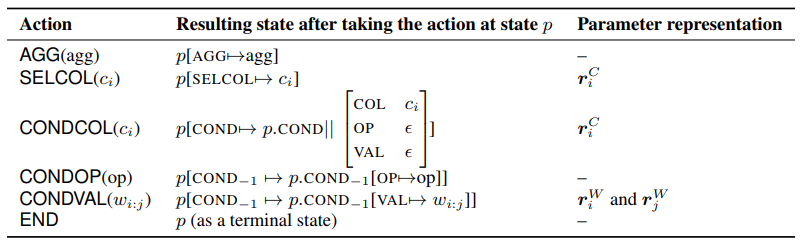
\includegraphics[width=20cm]{example/incsql.png}
%   \bicaption[这里将出现在插图索引中]
%     {中文题图}
%     {English caption}
%   \label{fig:SRR}
% \end{figure}

\subsection{动作序列}
\label{enl2sql:dzxl}

首先,我们给出对应于图\ref{fig:nl2sqlexample}中示例的完全解析之后的结构化表示:
% $\begin{Bmatrix}
%   1 & 2 \\
%   4 & 3 \\
% \end{Bmatrix}$
% \begin{bmatrix}
  
% \end{bmatrix}

$\begin{bmatrix}
  AGG    &  NONE  \\
  SELCOL &  Height(ft) \\
  COND   &   \langle
  % \begin{Bmatrix}
    \begin{bmatrix}
      COL  &  Name \\
      OP   &  =    \\
      VAL  &  “Willis Tower”\\
    \end{bmatrix}
    ,
    \begin{bmatrix}
      COL  &  Location \\
      OP   &  =    \\
      VAL  &  “Chicago”\\
    \end{bmatrix}
    % \end{Bmatrix}
    \rangle
  \end{bmatrix}$

因此,解析器的中间状态就被这样分部表示,其中一些尚未填充的特征值表示为$\epsilon$。
解析器的初始状态$p_{0}$的值为空和空列表,表示为$\begin{bmatrix}
  AGG    &  \epsilon  \\
  SELCOL &  \epsilon \\
  COND   &   \langle \rangle\\
  \end{bmatrix}$。

除此之外,我们还需要定义动作(action)清单。每个动作可以将解析器的状态从一个状态转换为另一个状态,即 $p \rightarrow p_{'}$ 。
我们设$p = \begin{bmatrix}
  AGG    &  agg  \\
  SELCOL &  selcol \\
  COND   &   cond\\
  \end{bmatrix}$,并且在表\ref{enl2sql:dzqd}中给出每个动作执行后的转移状态$p'$。

  \begin{table}[!hpb]
    \centering
    \bicaption[指向一个表格的表目录索引]
      {动作(action)清单}
      {A Table}
    \label{enl2sql:dzqd}
    \begin{tabular}{@{}llr@{}} \toprule
      % \multicolumn{2}{c}{Item} \\ \cmidrule(r){1-2}
      \textbf{动作(action)} & \textbf{由状态}$p$\textbf{执行该动作之后的状态} & \textbf{参数表示}\\\midrule
      % 1  & 	Q -> ( SClause ) ( ComplexCondition ) *\\
      AGG($agg$)  &  $p[AGG \mapsto agg]$  & - \\
      SELCOL($c_i$)  &  $p[SELCOL \mapsto c_i]$  & $r^C_i$ \\
      CONDCOL($c_i$)  &  $p[COND \mapsto p.COND||\begin{bmatrix}
        COL    &  c_i  \\
        OP &  \epsilon \\
        VAL   &   \epsilon\\
        \end{bmatrix}]$  &  $r^C_i$\\
      CONDOP(op)  &  $p[COND_{-1} \mapsto p.COND_{-1}[OP \mapsto op]]$  & -\\
      CONDVAL($w_{i:j}$)  &  $p[COND_{-1} \mapsto p.COND_{-1}[VAL \mapsto w_{i:j}]]$  &  $r^W_i and r^W_j$\\
      END  &  $p$(最终状态)  &  -\\\bottomrule
    \end{tabular}
  \end{table}

需要说明的是,在表\ref{enl2sql:dzqd}中,在解码器中所使用的参数表示将在\ref{enl2sql:decoder}节中进行解释;
$p[AGG \mapsto agg]$表示与状态$p$处于同一状态,不过其特征值$AGG$已经被赋值为$agg$;
$||$表示列表展开;$COND_{-1}$表示在列表中的上一个元素;


值得注意的是,动作$CONDVAL$会从输入问句$w$中选择所需的文字段$w_{i:j}$。
但这样做会导致一个问题,它将产生大量的动作,其数量级为问题长度的二次方。
因此,我们将动作$CONDVAL$分解为两个连续的子动作,一个去选择起始位置$w_i$,另一个则选择终止位置$w_j$。
在动作序列的最后,我们需要增加一个$END$动作来执行解析过程并使解析器进入结束状态。
举例来说,图\ref{fig:nl2sqlexample}中的例子可以看作是如下的一个动作序列:
\begin{enumerate}
  \item $AGG(NONE)$
  \item $SELCOL(c_3)$
  \item $CONDCOL(c_1)$
  \item $CONDOP(=)$
  \item $CONDVAL(w_{5:6})$
  \item $CONDCOL(c_2)$
  \item $CONDOP(=)$
  \item $CONDVAL(w_{8:8})$
\end{enumerate}
% ${AGG(NONE),SELCOL(c_3),CONDCOL(c_1),CONDOP(=),CONDVAL(w_{5:6}),CONDCOL(c_2),CONDOP(=),CONDVAL(w_{8:8})}$

该节中的定义是基于所有有效序列都具有AGG  SELCOL  (CONDCOL  CONDOP  CONDVAL)* END形式的假设之上。
也就保证了我们可以从所有的最终状态中提取出完整的逻辑形式出来。
对于其他不同结构的SQL语句来说,我们还需要重新设计动作的清单以及解析器的状态。


\subsection{编码器}
\label{enl2sql:encoder}

增强解析器模型的架构如图xx所示。

增强解析器模型包含编码器和解码器两个部分,其中编码器的具体步骤如下:
\begin{enumerate}
  \item 对于输入的句子$w$中的每个单词$w_i$,先将其使用词向量进行向量编码(word embedding[!!引用!!])。
  \item 将其送入一个双向的长短期记忆网络(bi-directional Long Short-Term Memory,简称bi-LSTM),其中每个细胞(cell)会有一个隐状态$h^W_i$。
  \item 由于一个列名可能由一个或多个单词构成,我们对每个列名先进行词向量编码并输入一个bi-LSTM中,再使用从bi-LSTM中得到的最终的隐状态作为列名初始表示(initial representation)。
  \item 使用自注意力机制(self-attention[!!引用!!])将该初始表示转换为$h^C_j$。
  \item 在得到基于内容的表示$h^W_i$和$h^C_j$之后,使用cross-serial dot-product attention[!!引用!!]得到$h^C_j$和$h^W_i$的加权平均值并作为单词$w_i$和$c_j$的上下文向量。
  \item 将这两个上下文向量进行拼接并分别送入使用自然语言问题和列名作为输入的bi-LSTM中。这两个LSTM网络的隐状态就是我们所期望的和上下文相关的表达$r^W_i$和$r^C_j$。
\end{enumerate}


\subsection{解码器}
\label{enl2sql:decoder}

在\ref{enl2sql:encoder}节中,我们已经获得了对于单词$w_i$上下文相关的表示$r^W_i$和以及列名$c_j$的上下文相关的表示$r^C_j$。
接下来是解码器部分的设计与细节。

首先,解码器的目标是为了对由输入$x$和历史活动$a_{<i}$构成的概率分布$P_{\theta}(a|x,a_{<i})$进行建模。其主要包括以下两点挑战:
\begin{enumerate}
  \item 活动(action)的不确定性:所有活动均需要取决于输入以及当前解析器的状态,不存在固定的活动。
  \item 解析器的决策完全依赖于上下文信息:解析器依赖于解码历史信息以及输入的问题和列名信息。
\end{enumerate}

为了解决第一个问题,我们使用了基于LSTM的解码器架构并使用活动的独立打分机制。
模型给每个候选的活动$a$打上分数$s_a$并且使用$softmax$函数将分数正则化(normalize)到一个概率分布上。
对于时刻$i$来说,我们用$h^{DEC}_i$来表示当前解码器的隐状态并且使用双线性函数$s_a = (h^{DEC}_i)^T U^A r^A_a$来给分数$a$建模。
双线性函数中$r^A_i$就是活动$a$的向量表示并且是由活动嵌入(action embedding)和参数表示(parameter representation)建模得到,
其中参数表示已经在表\ref{enl2sql:dzqd}中给出。

我们使用dot-product attention mechanism[!!引用!!]来捕获解析器的决策和输入的问题以及列名之间的依赖关系。
之后,将前一时刻$i$的输出活动表示$r^A_{a_i}$、自然语言问句的注意力向量$e^W_i$以及列名的注意力向量$e^C_i$拼接在一起,
作为$i+1$时刻的LSTM解码器的第一层的输入。
其中,向量$e^C_i = \sum_j \alpha_{i,j} r^C_j$,  $\alpha \propto h^{DEC}_i \cdot r^C_j$。
向量$e^W_i$的定义相似可得。



\subsection{解决ndo问题}
\label{enl2sql:ndo}

\subsection{解决过滤条件顺序问题}
\label{enl2sql:om}

\subsection{解决隐式列名问题}
\label{enl2sql:icn}

\section{实验与分析}
\subsection{数据集及评价指标}
\subsection{实验细节}
\subsection{实验结果}
\subsubsection{WIKISQL实验结果}
\subsubsection{对比试验结果}



\section{本章小结}